\documentclass[journal,12pt,twocolumn]{IEEEtran}
%
\usepackage{setspace}
\usepackage{textcomp}
\usepackage{gensymb}
%\doublespacing
\singlespacing

\usepackage[cmex10]{amsmath}
\usepackage{amsthm}
%\usepackage{iithtlc}
\usepackage{mathrsfs}
\usepackage{txfonts}
\usepackage{stfloats}
\usepackage{bm}
\usepackage{cite}
\usepackage{cases}
\usepackage{subfig}
%\usepackage{xtab}
\usepackage{longtable}
\usepackage{multirow}
%\usepackage{algorithm}
%\usepackage{algpseudocode}
\usepackage{enumitem}
\usepackage{mathtools}
\usepackage{steinmetz}
\usepackage{tikz}
\usepackage{circuitikz}
\usepackage{verbatim}
\usepackage{tfrupee}
\usepackage[breaklinks=true]{hyperref}
%\usepackage{stmaryrd}
\usepackage{tkz-euclide} % loads  TikZ and tkz-base
%\usetkzobj{all}
\usetikzlibrary{calc,math}
\usepackage{listings}
    \usepackage{color}                                            %%
    \usepackage{array}                                            %%
    \usepackage{longtable}                                        %%
    \usepackage{calc}                                             %%
    \usepackage{multirow}                                         %%
    \usepackage{hhline}                                           %%
    \usepackage{ifthen}                                           %%
  %optionally (for landscape tables embedded in another document): %%
    \usepackage{lscape}     
\usepackage{multicol}
\usepackage{chngcntr}
%\usepackage{enumerate}

%\usepackage{wasysym}
%\newcounter{MYtempeqncnt}
\DeclareMathOperator*{\Res}{Res}
%\renewcommand{\baselinestretch}{2}
\renewcommand\thesection{\arabic{section}}
\renewcommand\thesubsection{\thesection.\arabic{subsection}}
\renewcommand\thesubsubsection{\thesubsection.\arabic{subsubsection}}

\renewcommand\thesectiondis{\arabic{section}}
\renewcommand\thesubsectiondis{\thesectiondis.\arabic{subsection}}
\renewcommand\thesubsubsectiondis{\thesubsectiondis.\arabic{subsubsection}}

% correct bad hyphenation here
\hyphenation{op-tical net-works semi-conduc-tor}
\def\inputGnumericTable{}                                 %%

\lstset{
%language=C,
frame=single, 
breaklines=true,
columns=fullflexible
}
\newenvironment{amatrix}[1]{%
  \left(\begin{array}{@{}*{#1}{c}|c@{}}
}{%
  \end{array}\right)
}
\DeclarePairedDelimiter\abs{\lvert}{\rvert}%
\DeclarePairedDelimiter\norm{\lVert}{\rVert}%

% Swap the definition of \abs* and \norm*, so that \abs
% and \norm resizes the size of the brackets, and the 
% starred version does not.
\makeatletter
\let\oldabs\abs
\def\abs{\@ifstar{\oldabs}{\oldabs*}}
%
\let\oldnorm\norm
\def\norm{\@ifstar{\oldnorm}{\oldnorm*}}
\makeatother

\newtheorem{theorem}{Theorem}[section]
\newtheorem{problem}{Problem}
\newtheorem{proposition}{Proposition}[section]
\newtheorem{lemma}{Lemma}[section]
\newtheorem{corollary}[theorem]{Corollary}
\newtheorem{example}{Example}[section]
\newtheorem{definition}[problem]{Definition}
%\newtheorem{thm}{Theorem}[section] 
%\newtheorem{defn}[thm]{Definition}
%\newtheorem{algorithm}{Algorithm}[section]
%\newtheorem{cor}{Corollary}
\newcommand{\BEQA}{\begin{eqnarray}}
\newcommand{\EEQA}{\end{eqnarray}}
\newcommand{\define}{\stackrel{\triangle}{=}}
\bibliographystyle{IEEEtran}
%\bibliographystyle{ieeetr}
\providecommand{\mbf}{\mathbf}
\providecommand{\pr}[1]{\ensuremath{\Pr\left(#1\right)}}
\providecommand{\qfunc}[1]{\ensuremath{Q\left(#1\right)}}
\providecommand{\sbrak}[1]{\ensuremath{{}\left[#1\right]}}
\providecommand{\lsbrak}[1]{\ensuremath{{}\left[#1\right.}}
\providecommand{\rsbrak}[1]{\ensuremath{{}\left.#1\right]}}
\providecommand{\brak}[1]{\ensuremath{\left(#1\right)}}
\providecommand{\lbrak}[1]{\ensuremath{\left(#1\right.}}
\providecommand{\rbrak}[1]{\ensuremath{\left.#1\right)}}
\providecommand{\cbrak}[1]{\ensuremath{\left\{#1\right\}}}
\providecommand{\lcbrak}[1]{\ensuremath{\left\{#1\right.}}
\providecommand{\rcbrak}[1]{\ensuremath{\left.#1\right\}}}
\providecommand{\system}{\overset{\mathcal{H}}{ \longleftrightarrow}}
	%\newcommand{\solution}[2]{\textbf{Solution:}{#1}}
\newcommand{\solution}{\noindent \textbf{Solution: }}
\newcommand{\cosec}{\,\text{cosec}\,}
\providecommand{\dec}[2]{\ensuremath{\overset{#1}{\underset{#2}{\gtrless}}}}
\newcommand{\myvec}[1]{\ensuremath{\begin{pmatrix}#1\end{pmatrix}}}
\newcommand{\mydet}[1]{\ensuremath{\begin{vmatrix}#1\end{vmatrix}}}
%\numberwithin{equation}{section}
\numberwithin{equation}{subsection}
%\numberwithin{problem}{section}
%\numberwithin{definition}{section}
\makeatletter
\@addtoreset{figure}{problem}
\makeatother
\let\StandardTheFigure\thefigure
\let\vec\mathbf
\usepackage{mathtools, nccmath}
\begin{document}
\begin{center}
\huge Assignment 2\\
\large SUBHASISH SAIKIA\\
\large AI20MTECH14001\\
\end{center}
\vspace{0.5cm}
\begin{abstract}
This document explains the properties of a directional vector and how to find out if the given points are the vertices of a parallelogram, using directional vectors
\end{abstract}
\vspace{0.5cm}
Download all python codes from 
\begin{lstlisting}
https://github.com/subhasishsaikia22/EE5609-Matrix-theory
\end{lstlisting}
%
and latex-tikz codes from 
\begin{lstlisting}
https://github.com/subhasishsaikia22/EE5609-Matrix-theory
\end{lstlisting}
%
\vspace{0.5cm}
\section{Problem}
Using directional vectors, show that the points
\begin{align}
    \myvec{2 \\1},\quad \myvec{4 \\7} \quad \myvec{5 \\4}  \quad and \quad \myvec{1 \\4}
\end{align} 
are vertices of a parallelogram.
\section{Explanation}
Two lines are parallel if their respective directional vectors are in the same ratio.\\
Let the points be denoted by:
 \begin{align}
     \vec{A}= \myvec{2 \\1}\\
     \vec{B}= \myvec{5 \\4}\\
     \vec{C}=\myvec{4 \\7}\\
      \vec{D}=\myvec{1 \\4 }
 \end{align}
 The directional vector of $\vec{AB}$ is
\begin{align}
\myvec{2-5\\1-4}=\myvec{-3 \\-3}
\end{align}
The directional vector of $\vec{BC}$ is
\begin{align}
\myvec{5-4\\4-7}=\myvec{1 \\-3}
\end{align}
The directional vector of $\vec{CD}$ is
\begin{align}
\myvec{4-1\\7-4}=\myvec{3 \\3}
\end{align}
The directional vector of $\vec{AD}$ is
\begin{align}
\myvec{2-1\\1-4}=\myvec{1 \\-3}
\end{align}
The directional vector of $\vec{AC}$ is
\begin{align}
\myvec{2-4\\1-7}=\myvec{-2 \\-6}
\end{align}
Since the directional vectors of $\vec{AB}$ and $\vec{CD}$ are in the same ratio, so $\vec{AB}$ and $\vec{CD}$ are parallel and also opposite to each other.\\
Similarly, the directional vectors of $\vec{BC}$ and $\vec{AD}$ are in the same ratio,hence $\vec{BC}$ and $\vec{AD}$ are parallel and opposite.\\ 
Since the two pairs of opposite sides are parallel, the given points are the vertices of the parallelogram.\\

Moreover the sum of the directional vectors of $\vec{AB}$ and $\vec{BC}$ \\
  
\myvec{-3\\-3}+\myvec{1 \\-3}= \myvec{-3+1 \\-3-3}=\myvec{-2 \\-6}\\

Thus $\vec{AB}$ $+$ $\vec{BC}$= $\vec{AC}$, which satisfy
parallelogram law of vector addition i.e vector
sum of two adjacent side of a parallelogram is the
diagonal vector of the parallelogram.
\begin{figure}[!h]
 \centering
  \resizebox{\columnwidth}{!}{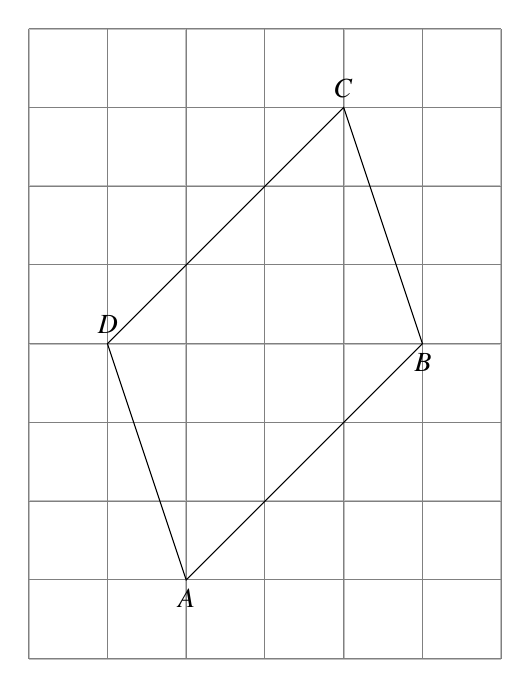
\begin{tikzpicture}
\tkzInit[xmin=0,xmax=6,ymin=0,ymax=8]
\tkzGrid[sub,color=gray, subxstep=2,subystep=2]
\tkzAxeXY[very thick]
\tkzGrid
    \coordinate (A) at (2,1);
    \coordinate (B) at (5,4);
    \coordinate (C) at (4,7);
    \coordinate (D) at (1,4);
    \draw (A)node[below]{$A$}--(B)node[below]{$B$}--(C)node[above]{$C$}--(D)node[above] {$D$}--cycle;
\end{tikzpicture}
}
    \caption{This is the parallelogram with the given vertices}
    \label{myfig:1}
\end{figure}
\end{document}
